\section{The New Small Wheel Detector}
\label{sec:nsw_detector}

In this section, a description of the NSW will be presented.
The layout of the NSW will be described in Section~\ref{sec:nsw_geo}
and then a description of the \micromegas (MM)~\cite{Giomataris:1995fq} and Small-strip Thin Gap Chamber (sTGC)
detector technologies that will compose the NSW
will be given in Sections~\ref{sec:nsw_mm} and \ref{sec:nsw_stgc}, respectively.
The MM are thought of as providing primarily high precision muon tracking
while the sTGC are thought of as primarily providing trigger primitives for the forward Level-1 muon trigger system.
As will be seen, though, both the MM and sTGC technologies will provide both high-quality tracking and trigger primitives.
The NSW must last for the remainder of the ATLAS detector's lifetime, throughout
both Run 3 and the entirety of the HL-LHC era.
In the following sections, the design decisions of the NSW --- related to both its layout 
and detector choices --- will be presented in light of their ability to address
the particular challenges described in the previous section.

%%%%%%%%%%%%%%%%%%%%%%%%%%%%%%%%%%%%%%%%%%%%%%%%%%%%%%%%%%%%%%%
% NSW GEO
%%%%%%%%%%%%%%%%%%%%%%%%%%%%%%%%%%%%%%%%%%%%%%%%%%%%%%%%%%%%%%%
\subsection{Geometry and Layout}
\label{sec:nsw_geo}

The NSW consists of 16 detector planes, separated into two `multilayers'.
Each multilayer will be composed of four detector planes of each of the two
detector technologies that make up the NSW: the Small-strip Thin Gap Chamber (sTGC)
and MicroMegas\footnote{The name `MicroMegas` is a loose acryonym for `MICROMEsh GAseous Structure'.} (MM)
detectors.
The sTGC are based on multiwire chamber technology, operated using CO$_2$:n-pentane gas mixture, and the MM are a type of
micropattern gaseous detector (MPGD)~\cite{MPGD}, operating using an Ar:7\%CO$_2$ gas mixture.
The detectors are arranged into sectors in azimuth, following a similar layout
as the current Small Wheel with alternating large and small sectors, as illustrated in Figure~\ref{fig:nsw_geo}.
The organisation of the detector technologies in each sector is illustrated in Figure~\ref{fig:nsw_sector_layout},
showing the sTGC--MM--MM--sTGC layout of the detector quadruplets, with a $50$\,mm spacer
frame separating the two halves.
Each sector of the NSW will have a length nearing 5\,m, giving the NSW a diameter of
nearly 10\,m.

The current Small Wheel muon system covers the range $1.0 < \lvert \eta \rvert < 2.7$, shown
in Figure~\ref{fig:muon_plan_view_eta}.
The NSW will not cover the entirety of this range, however, and will only cover the
range $1.3 < \lvert \eta \rvert < 2.7$ while the already-existing MDT chambers in the Small Wheel at $1.0 < \lvert \eta  \rvert < 1.3$
will remain in operation after the NSW installation.
The NSW will additionally extend the Level-1 muon trigger system acceptance to include
the region $2.4 < \lvert \eta \rvert < 2.7$, which is currently not the case.

The large number of detection planes provided by the NSW adds a large degree of redundancy
within each of the quadruplets of a given technology: if part of a layer, or even a complete layer,
is non-functioning the remaining layers within the quadruplet will compensate and a loss in performance
will be minimal.
There is additional redundancy provided by the fact that both MM and sTGC detector technologies
will be used for both tracking and trigger functionalities: if an entire or part of a quadruplet
becomes non-functioning, the tracking and/or trigger responsibilities of the lost detector
will be partially covered by the presence of the still-functioning quadruplet(s)/layer(s) of the other
detector technology covering the same or overlapping
$\eta$ range.
The degree of redundancy built into the NSW detector is such that the performance goals
of ATLAS with respect to the forward muon system can be met for the remainder of the experiment's
lifetime of 15 years or more.
With generally few opportunities for meaningful repair and maintenance access, this redundancy is
a necessity for these timescales.

\begin{figure}[!htb]
    \begin{center}
        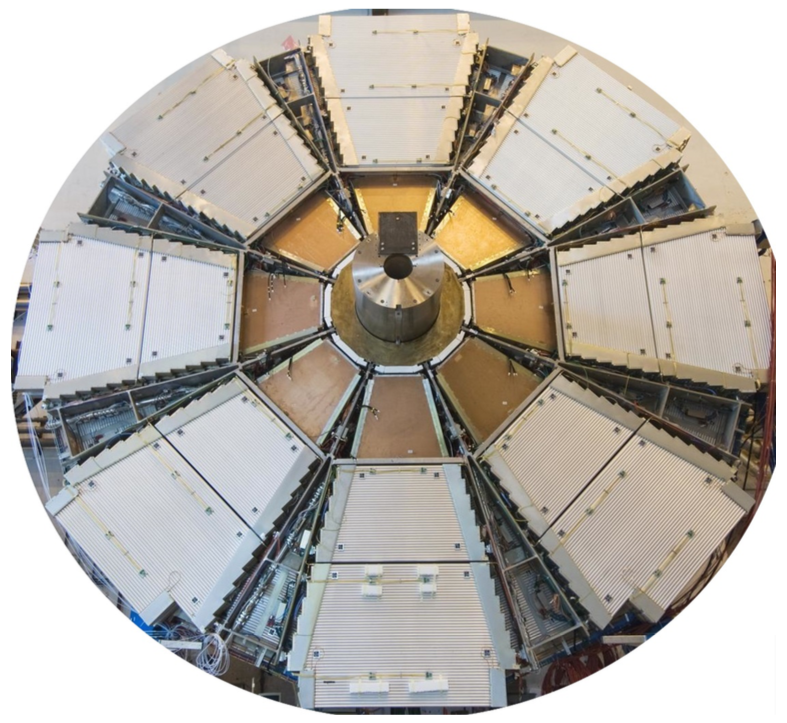
\includegraphics[width=0.48\textwidth]{figures/nsw/nsw_current_sw}
        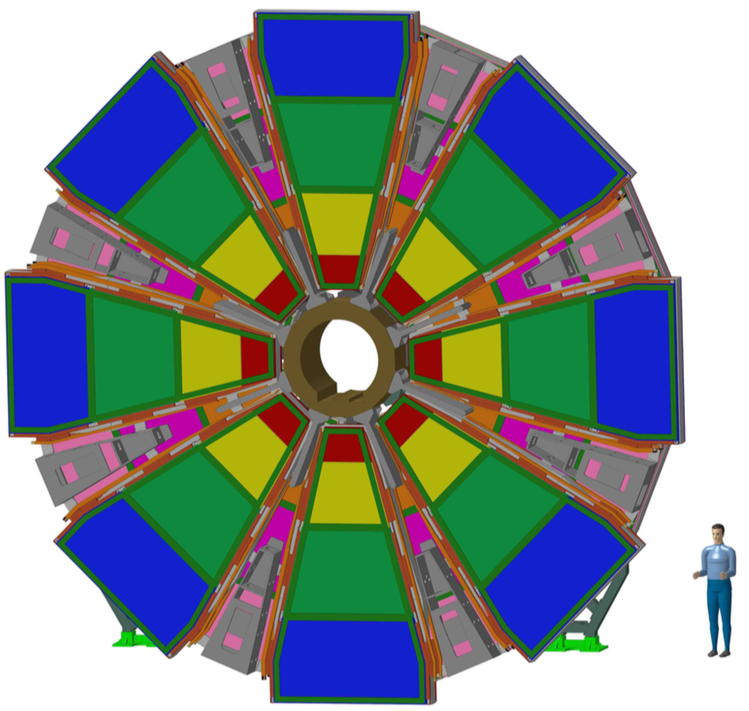
\includegraphics[width=0.48\textwidth]{figures/nsw/nsw_cartoon}
        \caption{
            \textbf{\textit{Left}}: Current Small Wheel detector (prior to installation in ATLAS), with CSC detectors (copper color) at low radii
                and MDT chambers (silver color) at higher radii.
            \textbf{\textit{Right}}: Geometry of the NSW, with a view of the large-sector side. The gaps in azimuth
                between the large sectors are instrumented with detectors on the side facing into the page.
        }
        \label{fig:nsw_geo}
    \end{center}
\end{figure}

\begin{figure}[!htb]
    \begin{center}
        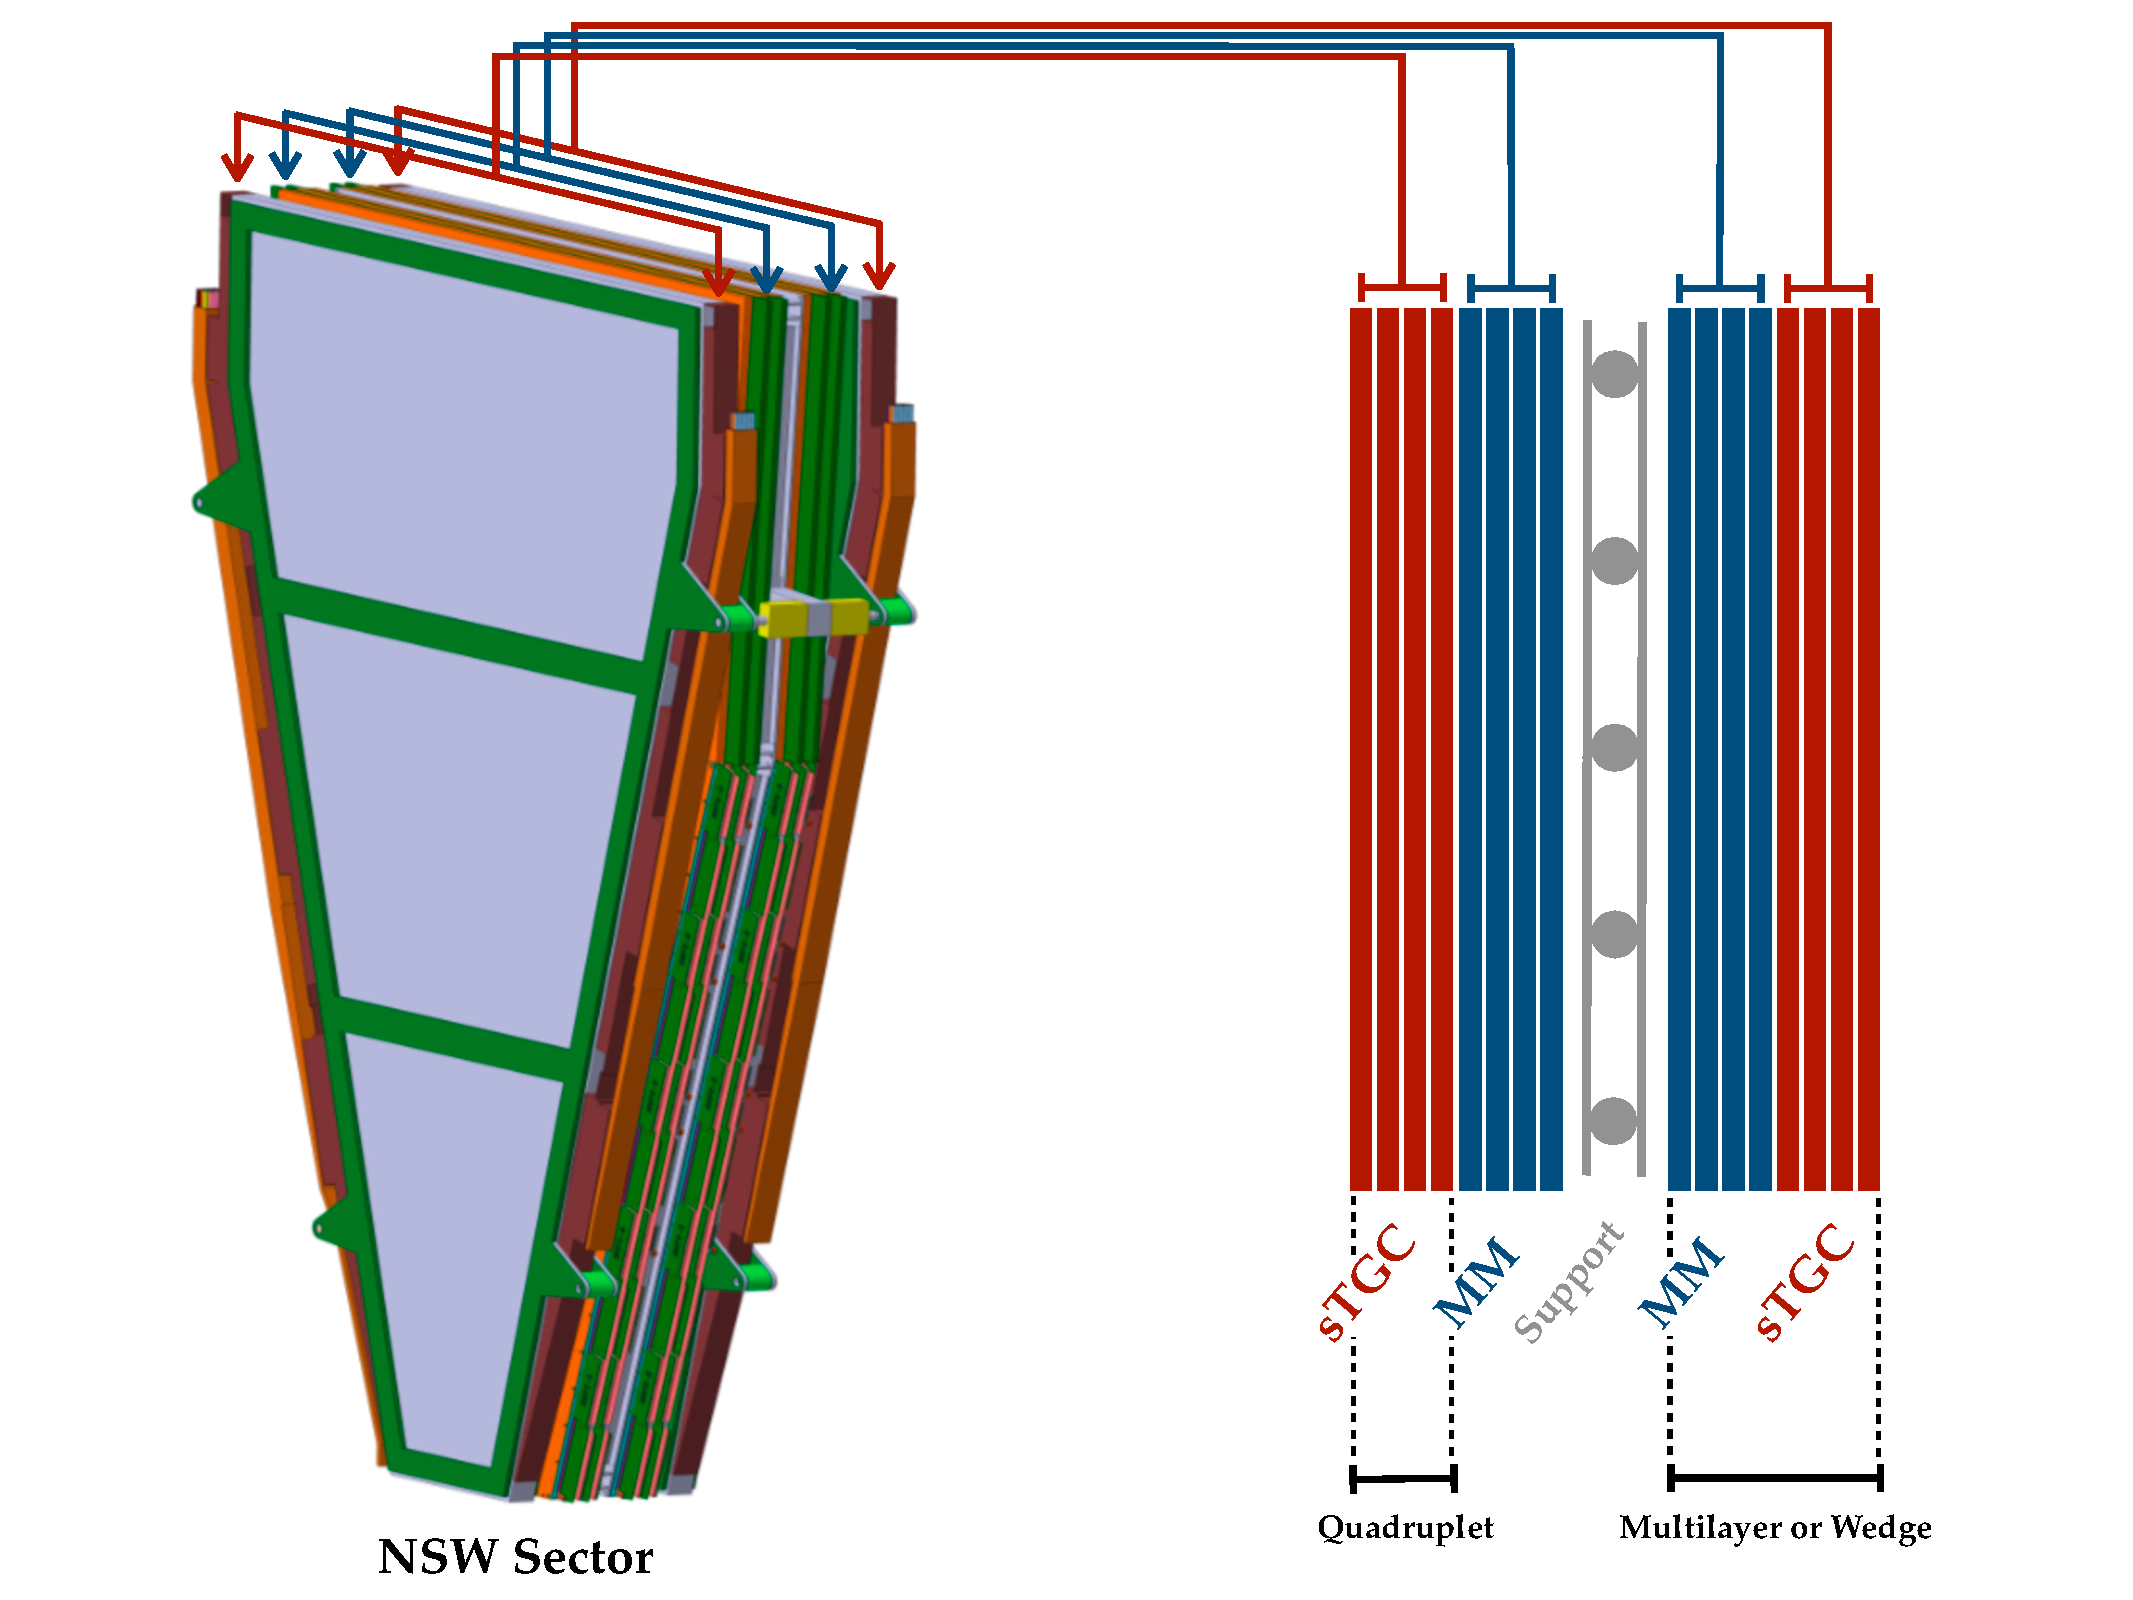
\includegraphics[width=0.8\textwidth]{figures/nsw/nsw_sector_layoutPDF}
        \caption{
            On the left is a mechanical drawing of an NSW sector, with the specific detector
            components illustrated on the right, composed of 16 detector planes: 8 MM layers
            sandwiched between 4 sTGC layers on either side.
            The base component of an NSW detector technology is a single detector plane,
            or layer, four of which are comprised in a single unit referred to as
            a `quadruplet'.
            A single side of the NSW, composed of an MM and sTGC quadruplet, is
            referred to as a `wedge' and a sector is referred to as a `double wedge'.
        }
        \label{fig:nsw_sector_layout}
    \end{center}
\end{figure}

%%%%%%%%%%%%%%%%%%%%%%%%%%%%%%%%%%%%%%%%%%%%%%%%%%%%%%%%%%%%%%%
% MICROMEGAS
%%%%%%%%%%%%%%%%%%%%%%%%%%%%%%%%%%%%%%%%%%%%%%%%%%%%%%%%%%%%%%%
\subsection{The Micromegas Detectors}
\label{sec:nsw_mm}

As mentioned above, the MM detectors are primarily designed with the high-precision tracking
requirements of the HL-LHC in mind, requiring a per-layer spatial hit resolution better than $100\,\micron$.
The MM detectors are characterised by readout strips with very fine segmentation and good
time resolution.
Due to this fine time resolution, they will be able to complement the trigger scheme based
on the sTGC detector technology.

MM detectors are characterised by two asymmetric regions.
The standard MM detector consists of a planar \textit{drift} electrode, a gas gap of
a few millimeters in thickness acting as a conversion and drift region, and a thin
metallic mesh at $\mathcal{O}(100)\,\micron$ above the readout electrodes.
The region between the mesh and readout electrodes is the amplification region wherein
gain factors on the order of $10^4$ are achievable.

The electric potentials within the drift and avalanche regions are maintained
at a few hundred V/cm and $\approx50$\,kV/cm, respectively.
Charged particles traversing the drift space ionise the gas and the electrons, liberated
in the ionisation process, drift towards the mesh at timescales on the order of tens of nanoseconds.
The electron avalanche takes place in the amplification region in about a nanosecond,
resulting in a fast current pulse on the readout electrode.

The MM detectors in the NSW are \textit{resistive-strip} MM detectors, characterised by an insulating
layer over the readout electrodes.
The insulating layer acts to protect the sensitive readout electrodes from sparking events that
reduce the detector performance over time and that are expected to happen frequently given
the very large gas amplification.
Resistive strips on top of the insulating layer collect the avalanche electrons and induce
signals on copper readout strips embedded beneath the insulating layer.
The geometry (strip pitch and width) of the copper readout strips need not necessarily be the
same as that of the resistive strips.
Resistive-strip MM detectors are able to sustain higher amplification and particle rates, a necessary
characteristic for targeting the high-luminosities foreseen at the HL-LHC.
The design and principle of operation of the resistive-strip MM technology is shown in Figure~\ref{fig:nsw_mm_principle},
in which incident MIPs traversing perpendicular and at an angle relative to the detector plane
are illustrated.

Each layer of an MM detector in the NSW is composed of $1024 \times 8$ parallel readout strips, giving
a highly granular spatial readout allowing for high resolution position measurements to be made.
Although all readout strips of a given MM layer are parallel, the MM quadruplets will be capable
of two-dimensional readout and will provide both $r$ and $\phi$ coordinate information
of traversing particles.
The two dimensional readout is achieved through the use of a small-angle stereo readout, in which
MM layers are tilted by fixed relative angles of $\pm 1.5$\,degrees.
This means of a two-dimensional readout is unlike that achieved by the CSC detectors in the current
Small Wheel, in which the readout plane consists of perpendicular wires and strips providing
the two dimensional readout information.
This perpendicular readout is susceptible to high rates of so-called \textit{ghost hits},
illustrated in the left side of Figure~\ref{fig:mm_stereo}, and leads to high levels of track-building ambiguities.
In the high particle rates expected at the HL-LHC, the multiplicities of these ghost hits would
lead to an unacceptable degradation in tracking performance.
The combination of the small-angle stereo readout and high strip-multiplicities on each MM layer will
enable the MM detectors to sustain these high particle rates.
In the right side of Figure~\ref{fig:mm_stereo}, the layout of the MM layers in the NSW as regards
their readout strip orientation (i.e. tilted or not) is illustrated.

Typical definitions of hit locations within strip-based detectors are based on the
centroid method, using the charge-weighted strip position to define the spatial location
of the hit.
This method works optimally for particles incident at angles perpendicular (zero inclination) to the detector readout plane.
The planar NSW detectors, however, will be subjected to particles originating from the IP that follow inclined tracks.
In the MM detectors, the centroid method provides worsening spatial resolution as the incident angles of these inclined tracks increase due
to the charges from the multiple ionisation events of a single incident particle being spread across multiple readout strips (Figure~\ref{fig:nsw_mm_principle}).
To overcome this, the MM hit reconstruction will use hit timing information
to use the $5$\,mm conversion gap as a time-projection chamber (TPC).
In the NSW, this two-dimensional TPC hit reconstruction is referred to as the micro-TPC (`$\mu$-TPC') reconstruction method.
The use of the timing information of each of the hits recorded by the readout strips
allows for the position above the readout plane to be reconstructed, thereby
allowing for a mini-track to be reconstructed that follows the ionisation history
of a single incident particle.
From this mini-track, a well-defined metric for defining the hit location for inclined tracks on
each MM layer can be defined, as illustrated on the left side of Figure~\ref{fig:mm_tpc_hit_loc}.
In the NSW, the MM hit location will be determined through the combined use of both the
charge-centroid and $\mu$-TPC methods, allowing for sufficient spatial resolution spanning the relevant
incident angles, as illustrated on the right side of Figure~\ref{fig:mm_tpc_hit_loc}.

\begin{figure}[!htb]
    \begin{center}
        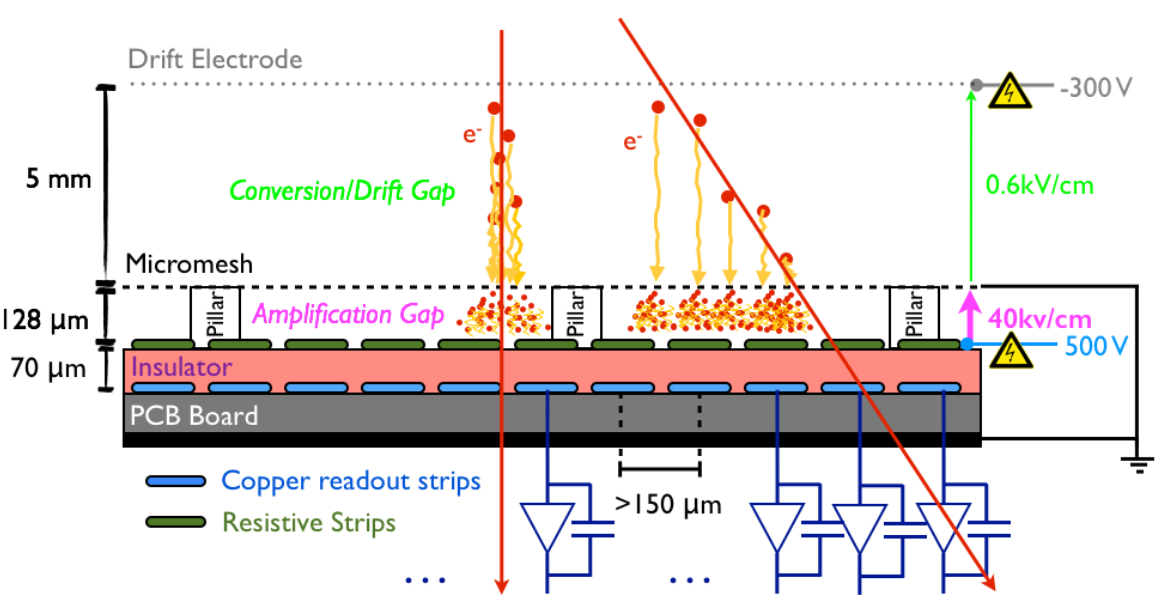
\includegraphics[width=0.75\textwidth]{figures/nsw/nsw_mm_principle}
        \caption{
            Illustration of the operating principle of a resistive-strip MM detector chamber.
            Figure taken from Ref.~\cite{NSWTDR}.
        }
        \label{fig:nsw_mm_principle}
    \end{center}
\end{figure}

\begin{figure}[!htb]
    \begin{center}
        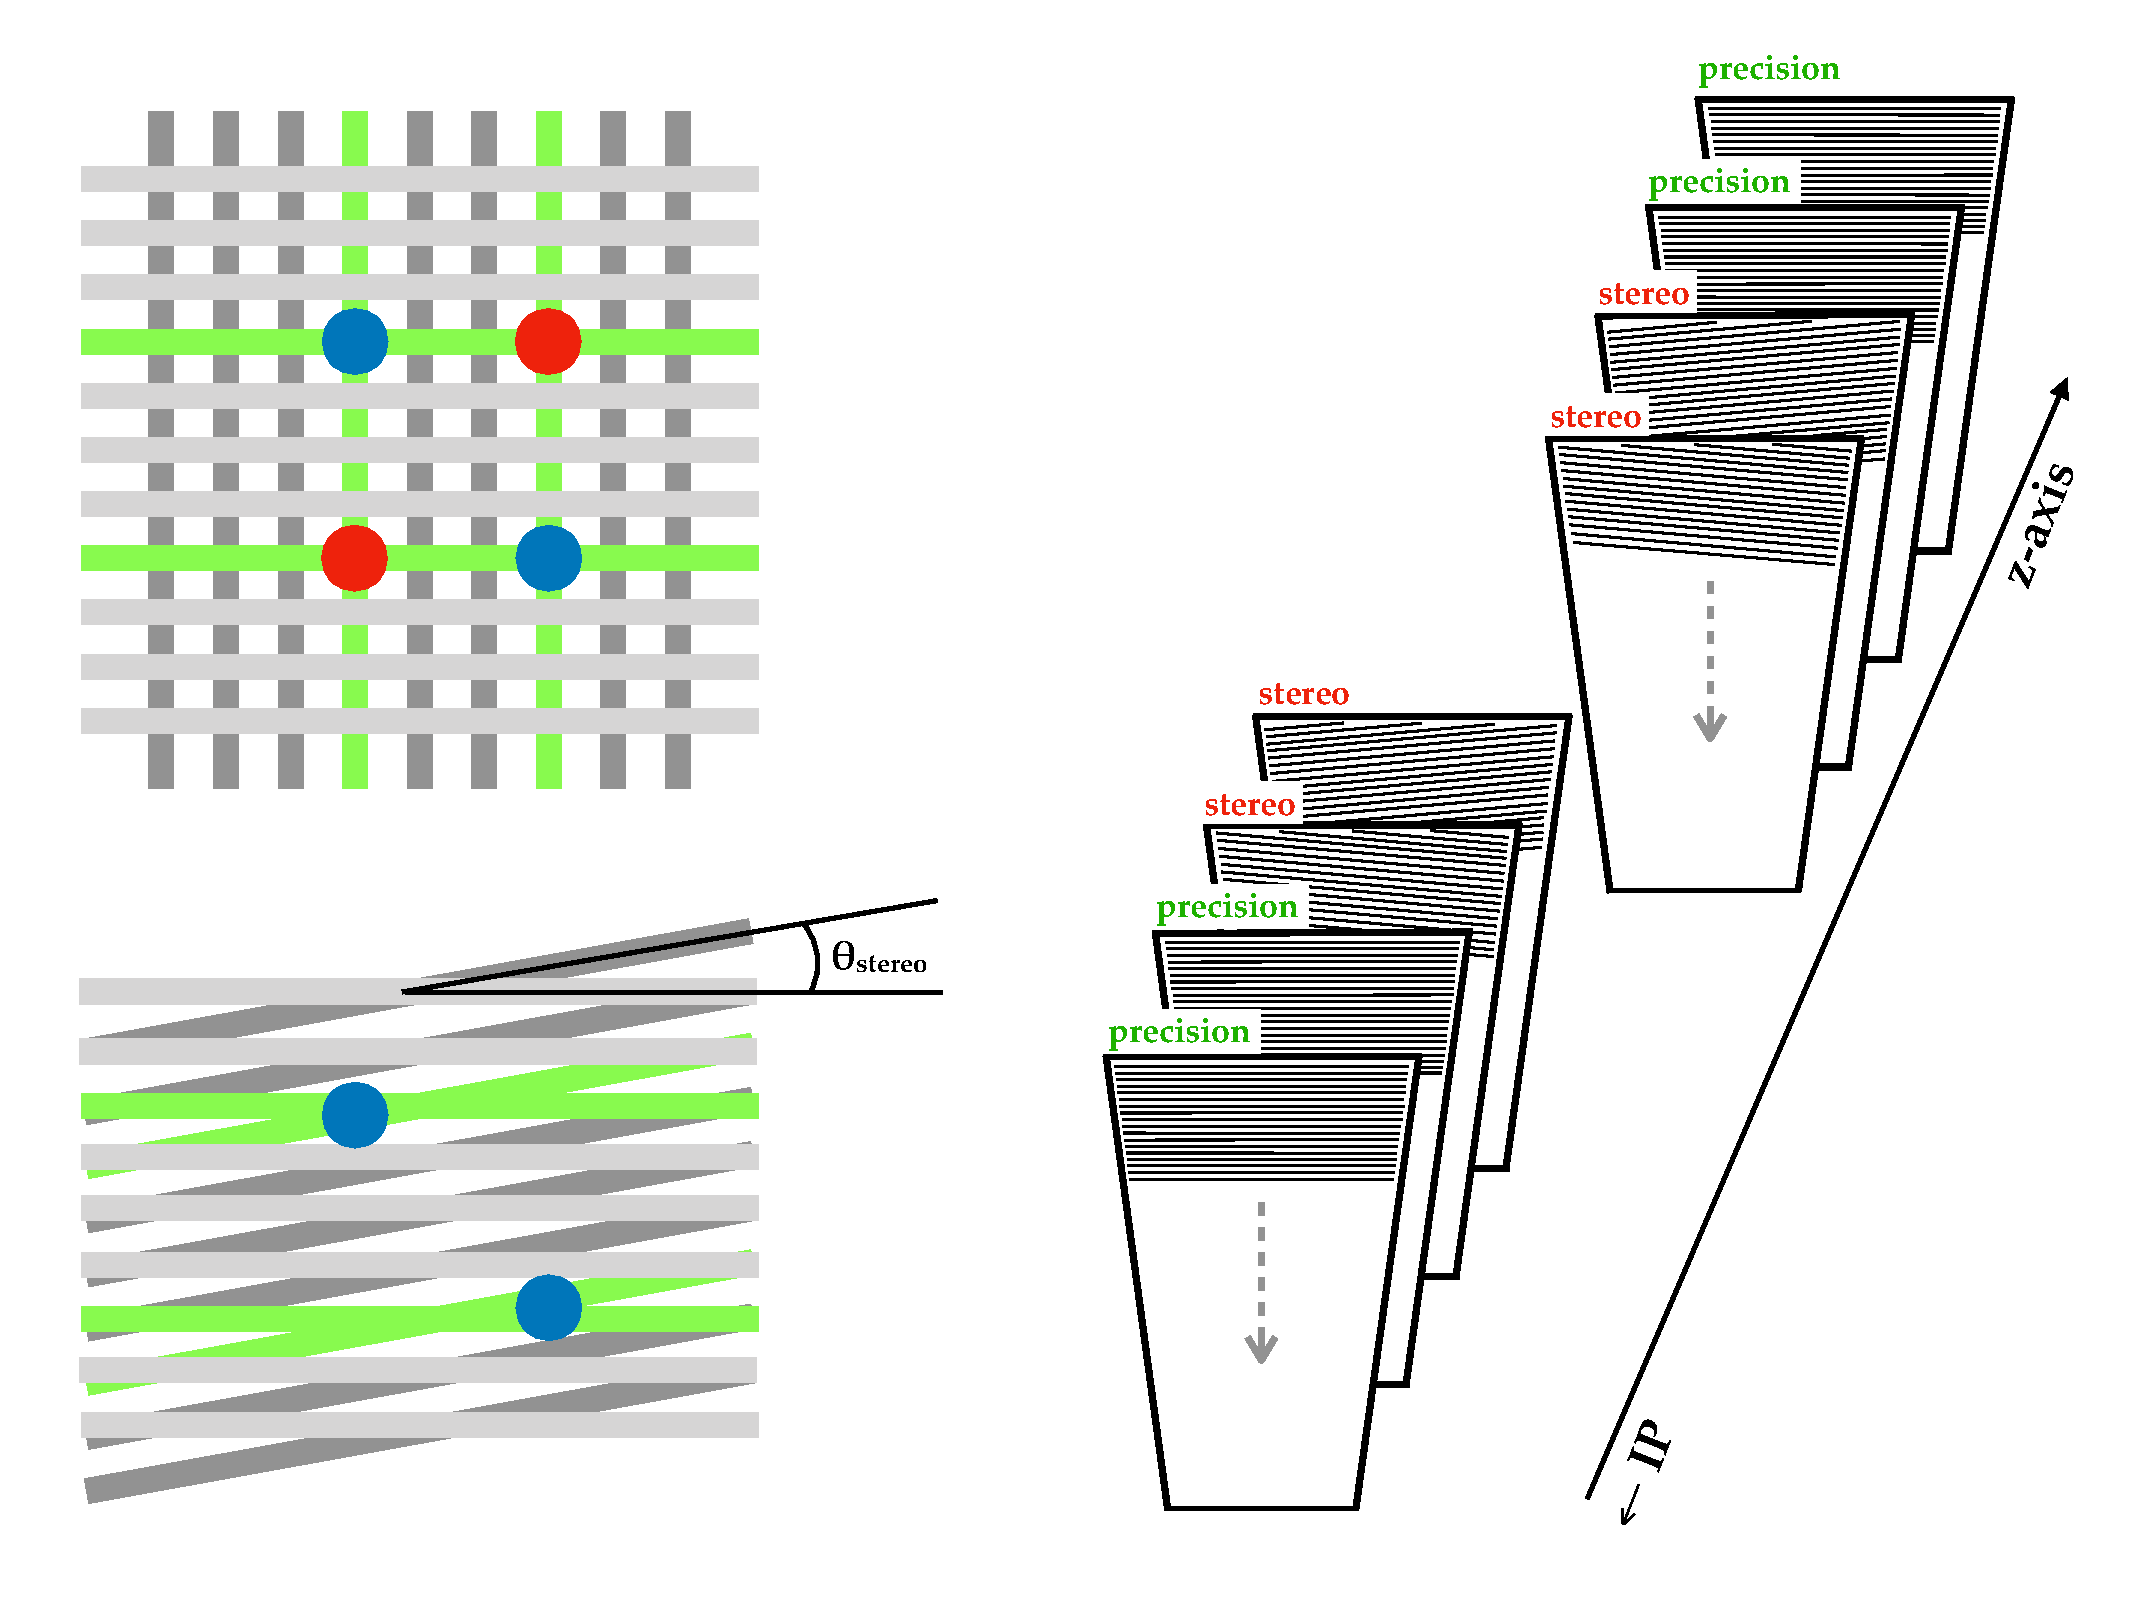
\includegraphics[width=0.8\textwidth]{figures/nsw/mm_stereo_cartoonPDF}
        \caption{
            \textbf{\textit{Left}}: Illustration of the small-angle stereo two-dimensional readout principle.
                The upper panel shows two layers with readout strips perpendicular to each other.
                The lower panel shows two layers with readout strips tilted at a small angle,
                $\theta_{\text{stereo}}$, relative to one another.
                In both cases, true detector hits are indicated by the blue dots.
                The readout strips registering the hits are indicated in green.
                In the case with perpendicular readout, there are two ghost hits indicated
                by the red dots.
                For perpendicular readout strips, there will generally be $N_{\text{ghost}} = (N^2 - N)$
                ghost hits for $N$ real hits when the readout strips on the two layers have
                equal pitches as in the case of the MM detectors in the NSW.
                On the lower panel, the green readout strips registering the two hits
                do not cross as a result of the small stereo angle and there are no ghost hits.
            \textbf{\textit{Right}}: Illustration of the layout of the `precision' and `stereo'
                readout layers of the two MM quadruplets in a given NSW sector.
                The precision layers, so-called since their readout strips are along $\phi$ and measure directly the
                coordinate in the bending plane of passing muons relevant for \pT~determination, are the outer two layers of
                each quadruplet relative to the spacer frame.
                The stereo layers are those with the readout strips tilted at $\pm 1.5^{\degree}$ relative to the precision layers and are the two layers
                in each quadruplet nearest the central spacer frame.
                One stereo layer in each quadruplet has stereo angle $+1.5^{\degree}$ and the other $-1.5^{\degree}$, making
                for $\Delta \theta = 3^{\degree}$ between the two stereo layers in each quadruplet.
        }
        \label{fig:mm_stereo}
    \end{center}
\end{figure}

\begin{figure}[!htb]
    \begin{center}
        \raisebox{1.4cm}{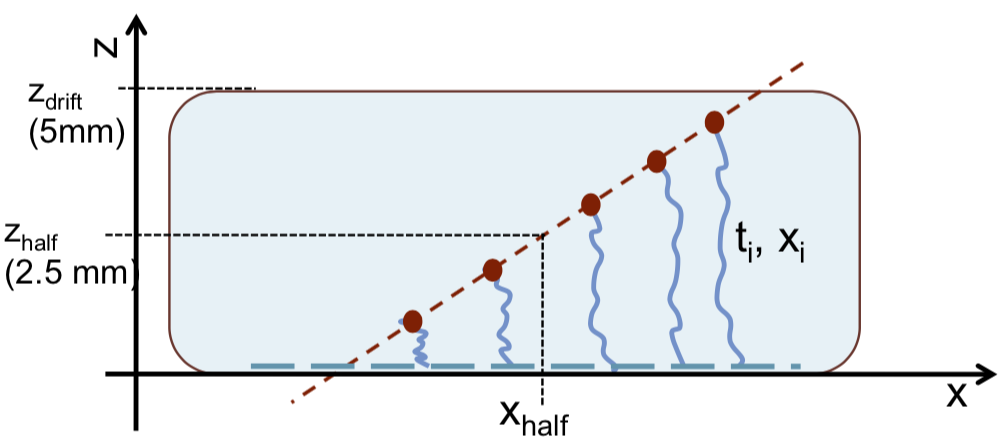
\includegraphics[width=0.48\textwidth]{figures/nsw/mm_tpc_hit_loc}}
        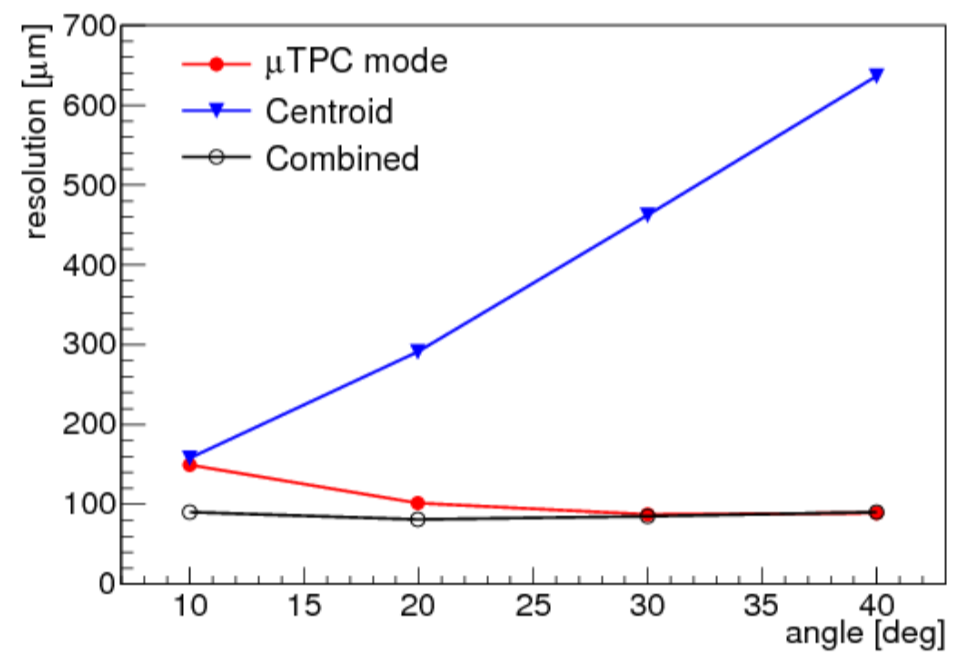
\includegraphics[width=0.48\textwidth]{figures/nsw/tpc_vs_centroid_res}
        \caption{
            Figures taken from Ref.~\cite{NSWTDR}.
            \textbf{\textit{Left}}: Illustration of the `$x_{\text{half}}$' method of defining a hit position for
                an inclined track: the hit position is defined as the position on the readout plane
                corresponding to the half-height location along the reconstructed tracklet in the MM conversion gap.
            \textbf{\textit{Right}}: Expected MM spatial resolution with charge centroid method (blue triangles), $\mu$-TPC
                method (filled red circles), and the combination of the two (black open circles) as a function
                of particle incident angle.
                The combination of the two methods achieves the greater-than $100\,\micron$ single-layer spatial resolution
                required for HL-LHC operation for the expected range of incident angles.
        }
        \label{fig:mm_tpc_hit_loc}
    \end{center}
\end{figure}

%%%%%%%%%%%%%%%%%%%%%%%%%%%%%%%%%%%%%%%%%%%%%%%%%%%%%%%%%%%%%%%
% STGC
%%%%%%%%%%%%%%%%%%%%%%%%%%%%%%%%%%%%%%%%%%%%%%%%%%%%%%%%%%%%%%%
\subsection{The Small-strip Thin Gap Chamber Detectors}
\label{sec:nsw_stgc}

The sTGC are those detectors stated as being primarily used for producing trigger primitives
to be used by the Level-1 muon trigger system.
As triggering detectors, they have fast signal formation and readout times owing to their characteristic high
operating electric fields.
This enables
them to provide accurate bunch crossing identification (i.e. assigning hits to a specific bunch crossing).
The average drift time of ionisation electrons within the sTGC chambers is less than 25\,ns,
with the earliest cluster arrival times well below 10\,ns.
Figure~\ref{fig:stgc_timing} shows the distribution of the measured drift times in an
sTGC, with 95\% of the measured and simulated data being inside a 25\,ns (the LHC bunch crossing
frequency) time window.
The sTCG detectors also provide good online angular resolution --- better than 1\,mrad --- for the track segments
reconstructed across the layers of an sTGC quadruplet, meaning fairly good spatial resolution.
The high quality angular resolution allows for good \pT~determination based on the trigger primitives
provided to the Level-1 trigger.
Offline spatial reconstruction for track segments provided by the sTGC detectors will also be good, matching
the sub-100$\,\micron$ threshold for the HL-LHC precision tracking requirements in the forward region
of the muon system.

\begin{figure}[!htb]
    \begin{center}
        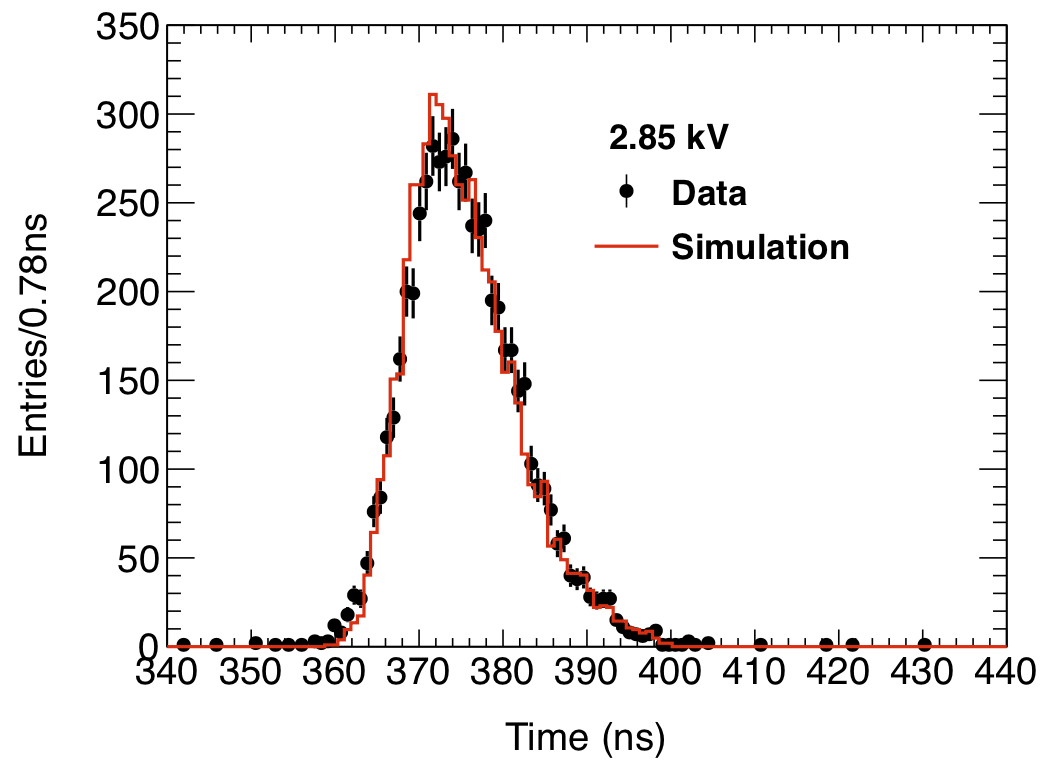
\includegraphics[width=0.5\textwidth]{figures/nsw/stgc_timing}
        \caption{
            Due to the very thin gap and the intense electric field applied,
            $\approx95$\,\% of the measured drift times of passing MIPs are
            confined within a window of 25\,ns, showing that the sTGC
            are capable of reliable bunch crossing assignment.
            Figure taken from Ref.~\cite{NSWTDR}.
        }
        \label{fig:stgc_timing}
    \end{center}
\end{figure}

The basic sTGC detector is shown in Figure~\ref{fig:stgc_drawing}.
It consists of a grid of $50\,\micron$ gold-plated tungsten wires with $1.8$\,mm pitch
sandwiched between two cathode planes at a distance of $1.4$\,mm.
On one plane there are the readout pads and on the other the strips.
The strips have a $3.2$\,mm pitch, which is smaller than that of the current TGC
detectors used in the current forward muon system (Figure~\ref{fig:muon_plan_view_eta}),
which is the origin of the name of the sTGC detectors.
The wires and strips are perpendicular, with the wires stretching along $r$ and the
strips along $\phi$.

The pads are used to form coincidences between the layers of the sTGC quadruplets in order
to form projective trigger primitives corresponding to muon tracks pointing roughly back to the IP.
There are $\approx 1300$ pads per sTGC layer.
The collected charge from all components of the sTGC --- the pads, strips, and wires --- associated with a traversing particle are read out and
used for the subsequent offline precision muon-track reconstruction.
Two-dimensional readout is achieved by the $r$ and $\phi$ information provided by the strips
and wires, respectively.
To help cope with the foreseen high particle rates, and to reduce the types of tracking ambiguities
described in Section~\ref{sec:nsw_mm} due to combinatorial hits, only
those wires and strips covering the projective area of pads registering the passage of
the particle are read out.
Additionally, wires are grouped together (i.e. multiple wires correspond to a single readout
channel) as only a rough measurement of the azimuthal coordinate --- not relevant for \pT~determination in the trigger---
is needed.
With the charge information collected from the three sub-components, the sTGC is able to achieve very
good spatial resolutions approaching $\approx 80\,\micron$ ($\approx 100\,\micron$) per layer for perpendicular (inclined) tracks.

\begin{figure}[!htb]
    \begin{center}
        \raisebox{0.8cm}{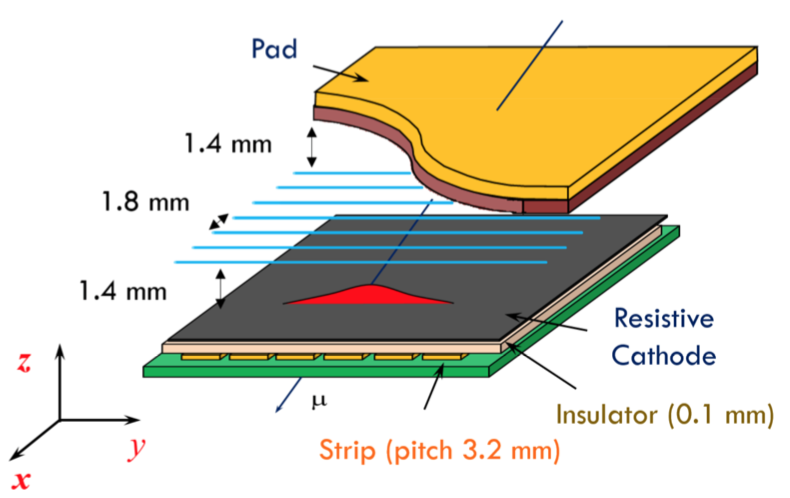
\includegraphics[width=0.52\textwidth]{figures/nsw/stgc_drawing}}
        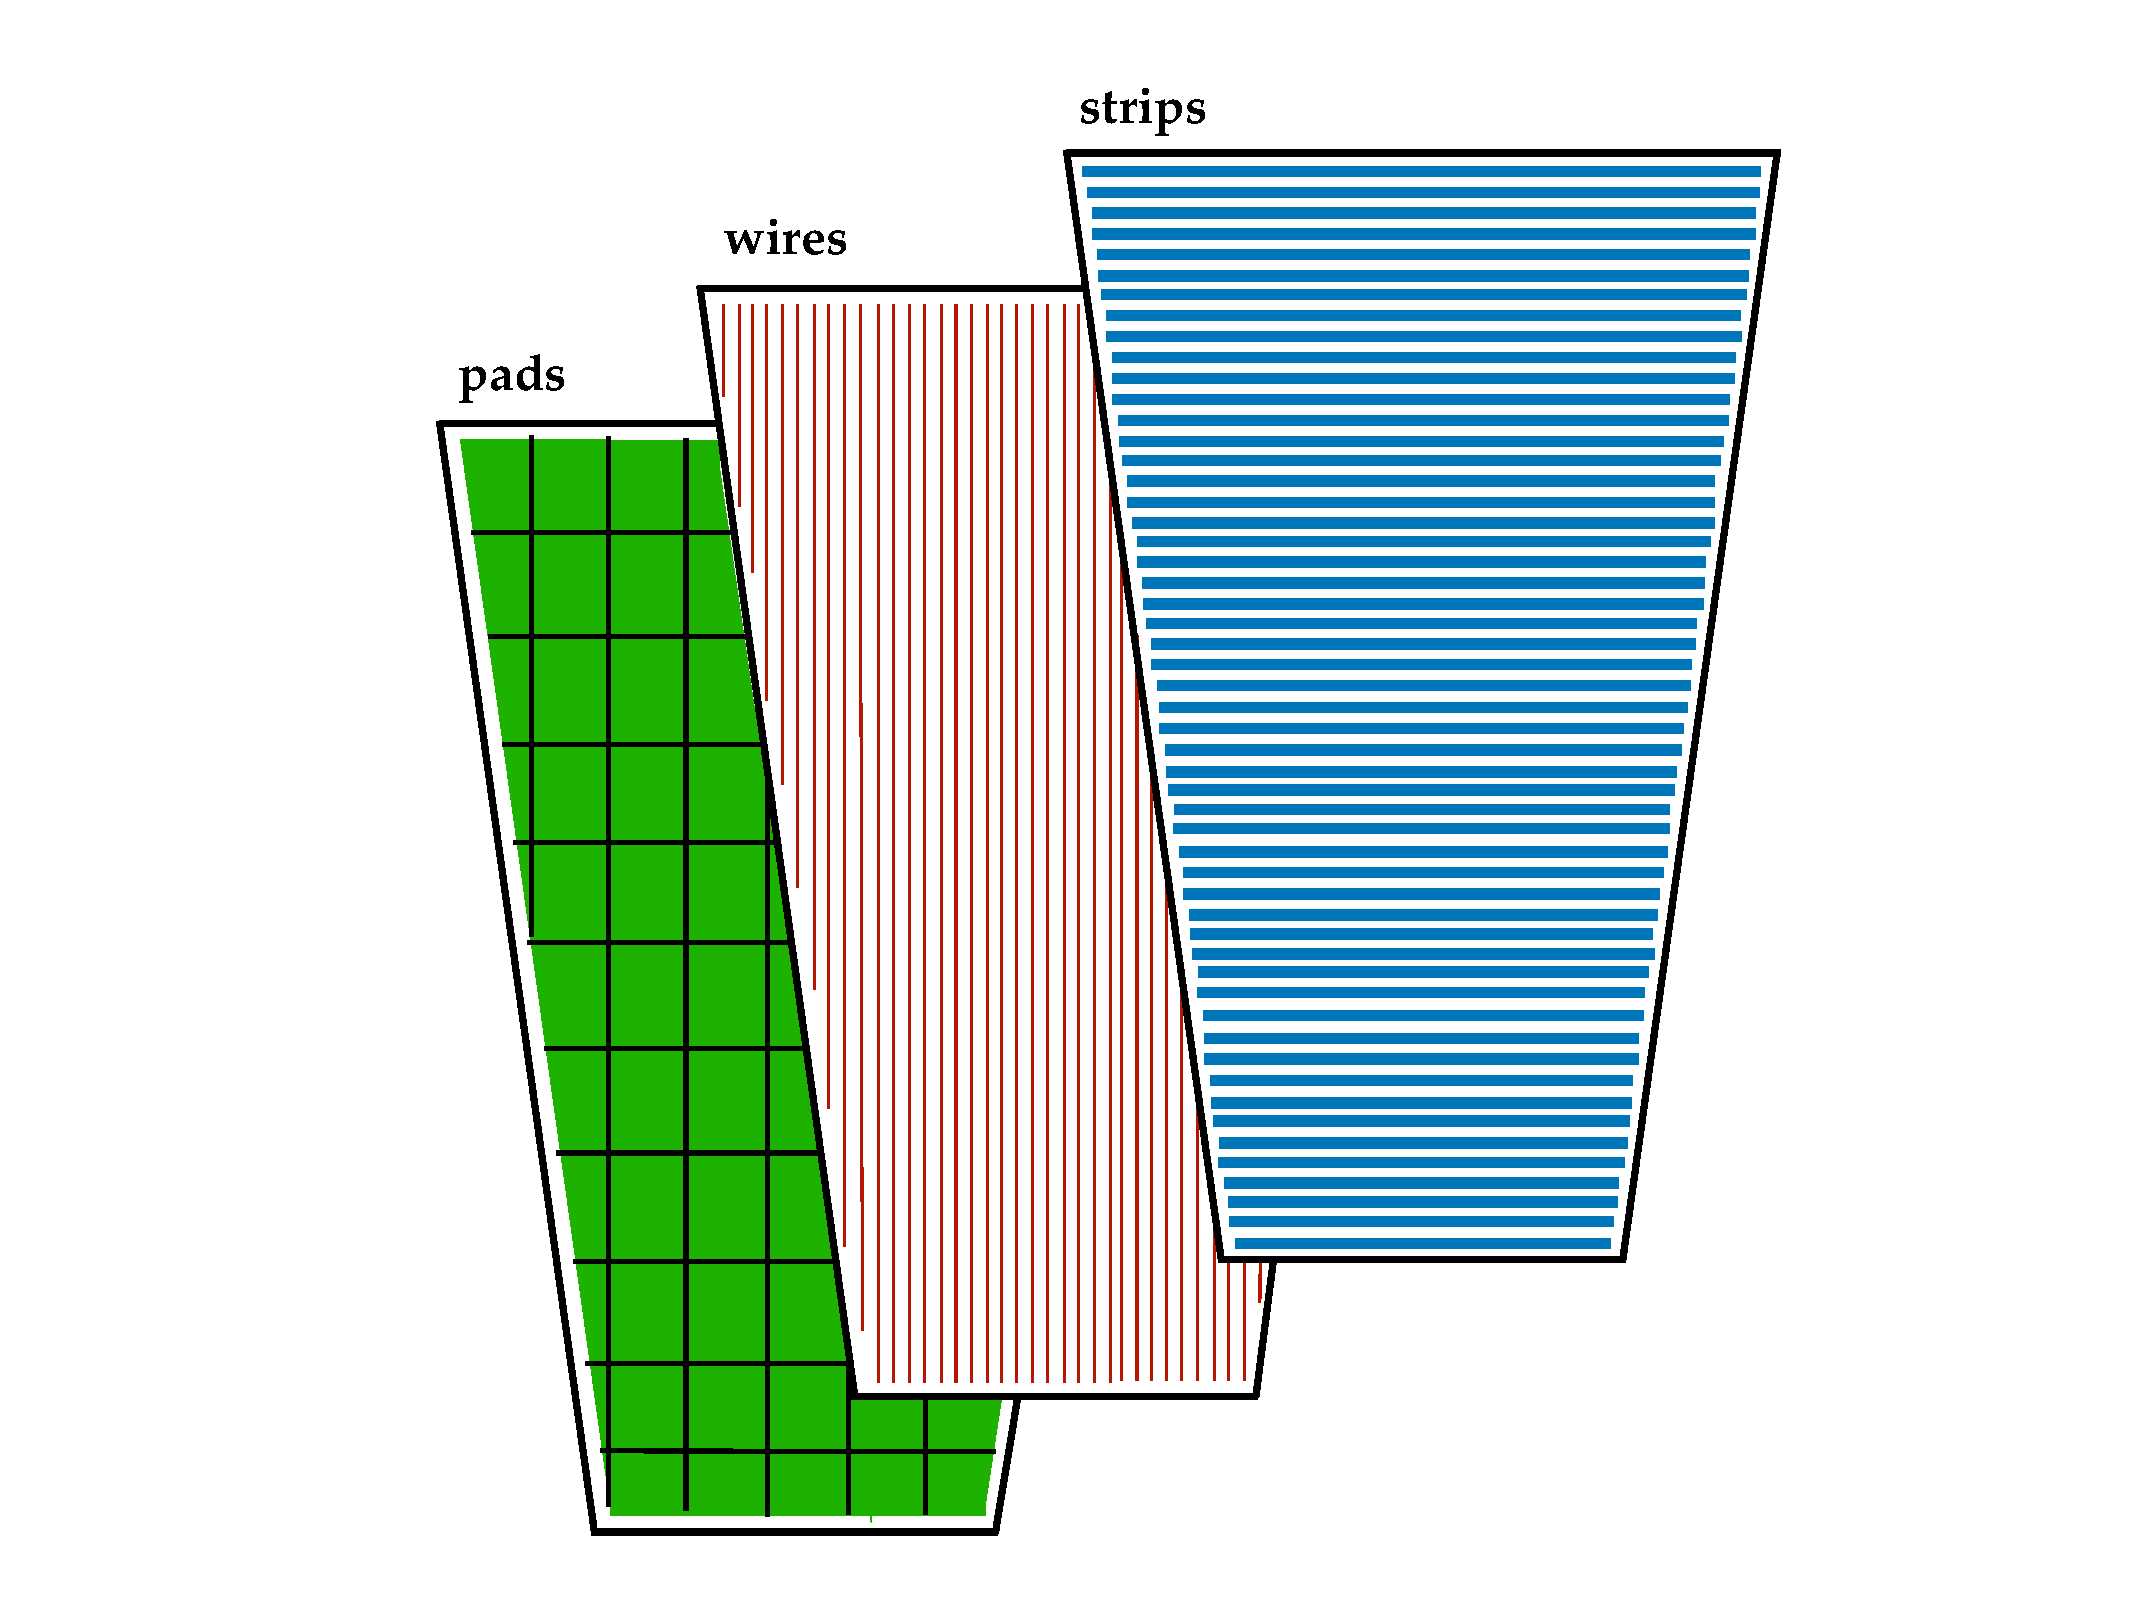
\includegraphics[width=0.45\textwidth]{figures/nsw/stgc_layer_cartoonPDF}
        \caption{
            \textbf{\textit{Left}}: Graphical representation of the internal structure of an
                sTGC detector.
                The passage of a traversing MIP (black line) induces signals on the anode wires, readout pads,
                and strips behind the resistive cathode planes as a result of the drifting of ionisation
                charges and their subsequent multiplication (in red).
            \textbf{\textit{Right}}: Illustration of the geometry of the sTGC pads, wires, and strips and their
                relative layout in a single sTGC layer.
                The strips (blue) are along $\phi$ and provide the measurement of the precision momentum coordinate
                in the particle bending plane.
                The wires are along $r$ and provide measurements sensitive to $\phi$.
                The pads provide information necessary for building trigger coincidences between
                the layers of an sTGC quadruplet and determine which subset of wires and strips will
                subsequently be readout upon a Level-1 trigger accept.
                The drawing is not to scale and does not illustrate the actual segmentation
                of the readout components in a given layer, only their relative orientation.
        }
        \label{fig:stgc_drawing}
    \end{center}
\end{figure}
